\documentclass{article}

\usepackage[utf8]{inputenc}
\usepackage[T1]{fontenc}
\usepackage{amsmath}
\usepackage{booktabs}
\usepackage{tikz}
\usepackage{pgfplots}
\pgfplotsset{compat=1.18}
% \usepackage{lipsum}

\title{TeXtra Test Document}
\author{Test}
\date{\today}

\begin{document}

\maketitle

% Simple supply and demand tikz graph
\begin{figure}
	\centering
	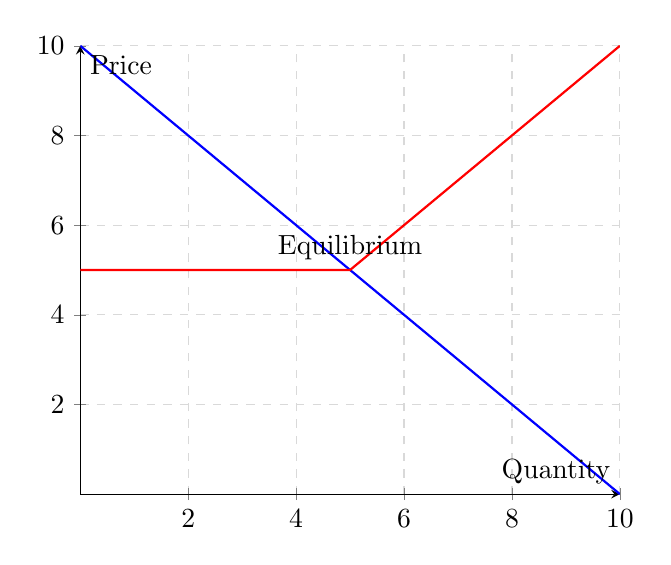
\begin{tikzpicture}
		\begin{axis}[
			xlabel={Quantity},
			ylabel={Price},
			xmin=0, xmax=10,
			ymin=0, ymax=10,
			axis lines=middle,
			grid=both,
			grid style={dashed, gray!30},
			]
			\addplot[blue, thick] coordinates {(0,10) (5,5) (10,0)};
			\addplot[red, thick] coordinates {(0,5) (5,5) (10,10)};
			\addplot[black, thick] coordinates {(5,5)};
			\node at (axis cs:5,5) [above] {Equilibrium};
		\end{axis}
	\end{tikzpicture}
	\caption{Supply and Demand Graph}
	\label{fig:supply-demand}
	\caption{}\label{fig:fig1}
\end{figure}

Now, I will create a simple circle in tikz:
\begin{figure}
	\centering
	
\begin{tikzpicture}
		\draw (0,0) circle (1cm);
	\end{tikzpicture}
	\caption{}\label{fig:fig2}
\end{figure}


\begin{itemize}
	\item Item
\end{itemize}

This is a simple test document. Edit the text and compile it in TeXtra to check that the editor and PDF preview are working.

Here is I want more text. Lorem ipsum dolor sit amet, consectetuer adipiscing elit. Ut purus elit, vestibulum ut, placerat ac, adipiscing vitae, felis.
	
\begin{itemize}
	\item Test
	\item Test 2
\end{itemize}

\section{Section}
Lorem ipsum dolor sit amet.

\subsection{Subsection}

\begin{table}[htbp]
	\centering
	\caption{}\label{tab:tab1}
	\begin{tabular}{lcc}
		\toprule
		Variable & (1)  & (2)  \\
		\midrule
		A        & 0.00 & 0.00 \\
		B        & 0.00 & 0.00 \\
		\bottomrule
	\end{tabular}
\end{table}


\begin{equation}
	Y = aX + b + \varepsilon \label{eq:slope}
\end{equation}

% TODO: description
% FIXME: Something


Reference equation~\eqref{eq:slope}.


\end{document}
